\chapter{User Guide}
\label{userguide}
In this appendix, we provide a user guide for running the interface on own infrastructure or simply using it for e-mail management.

The appendix is separated into two sections. The first section describes the interaction with the interface on the end user's level. The second section details the API library, and explains how to run the interface on a UNIX server.

\section{Interface interaction}
KamehaMail can be tried on the webpage \texttt{hruska.blesmrt.cf/KamehaMail} using any reasonable modern web browser. The main page is a simple login panel with sign up option. To registrate, go to the \texttt{Sign Up} option, choose a username (with domain at the end, in this case \texttt{@hruska.blesmrt.cf}).

After successful login, the e-mails page shows up. There are several points of interest:

\paragraph{Left navigation panel.}
Left navigation panel contains tags for e-mails. First four tags are system tags, \texttt{Inbox}, \texttt{Archive}, \texttt{Trash} and \texttt{Sent}. After them comes menu with customisable user-defined tags\footnote{list of possible icons for tags can be found on \texttt{https://material.io/tools/icons/}}. There is a possibility to create a search tag from the current search.

\paragraph{Top bar.}
The top bar contains search panel (center) and account management menu (right). Possible queries for the search are the following:
\begin{itemize}
\item User can simply type the term he is searching for. In this case, the search engine will look into all analyzed fields for the match.
\item User can specify the search field, for example \texttt{subject: Hello}. Possible search fields are \texttt{subject}, \texttt{text}, \texttt{from} and \texttt{to}
\item There is one more unanalyzed search field named \texttt{tag}. Any system or user-defined tags can be searched using the same syntax (e.g \texttt{tag: inbox}).
\item User can filter the results by date. Date value must be in \texttt{time: dd/mm/yyyy} or \texttt{time: dd.mm.yyyy} format. Possibilities of date filtering are:
\begin{itemize}
\item lesser than \texttt{time: <date}
\item greater than \texttt{time: >date}
\item between \texttt{time: date-date}
\item exact date \texttt{time: date}.
\end{itemize}
\end{itemize}
All of the queries above can be combined using \texttt{and}, creating multi-criteria queries with any number of white spaces in between.
Account management provides options for password change, mailer change and logout.

\paragraph{Center.}
The button in the bottom right corner opens a form for writing a new e-mail. It features text editor and a file drop for attachments.

The center contains grouped e-mails. Each group indicates the number of the e-mails it references to and the subject of the conversation. If the subject is in bold, one or more messages in the conversation are new (i.e. unread). The tag buttons are to the right of the subject: mark read/unread, archive, delete and a drop-down menu for user's tags.
Preview of each e-mail is shown once the group is opened. Each e-mail group provides text editor and \texttt{Quick Reply} option to reply directly to the conversation. Reply and forward options on the right side of each e-mail open a new prefilled form for sending.

All basic features are displayed in \autoref{fig:menu}.
\begin{figure}
\centering
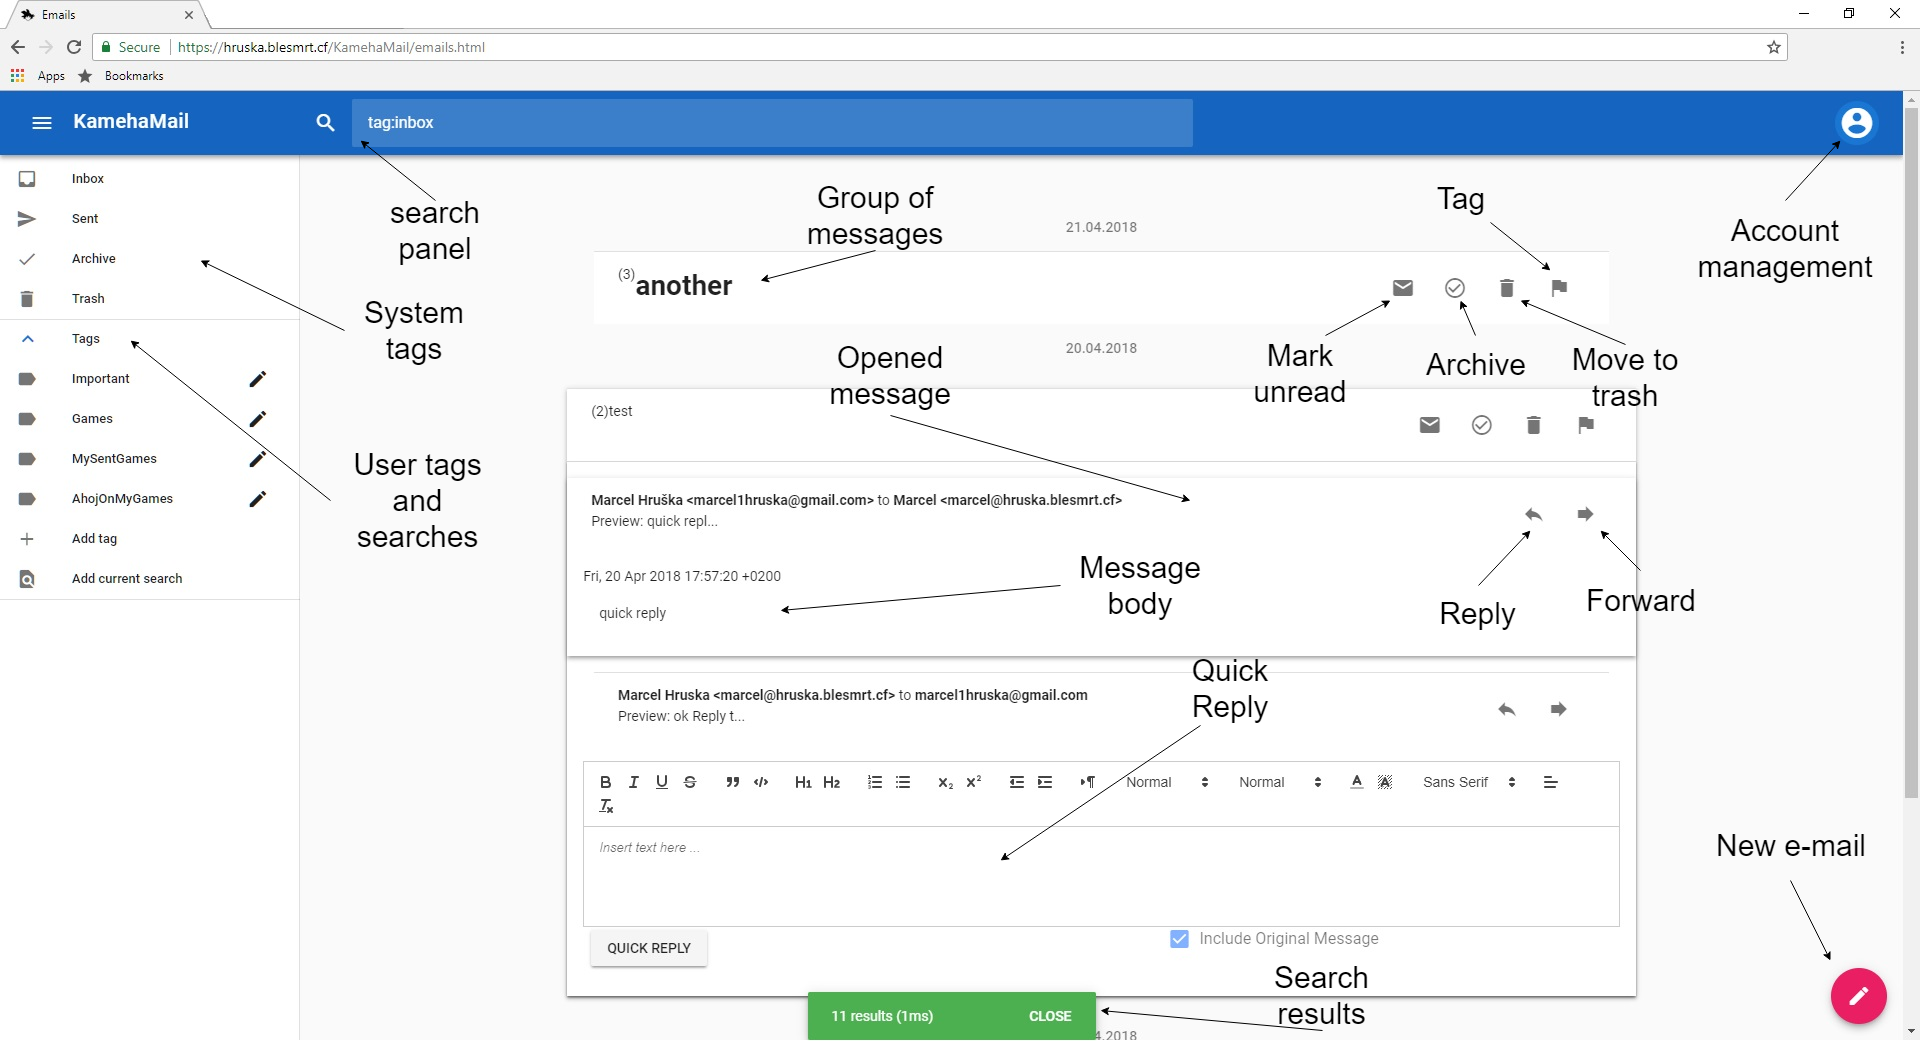
\includegraphics[width=\textwidth]{img/menu.png}
\caption{Main menu description.}
\label{fig:menu}
\end{figure}

\section{Server configuration}

We briefly cover the installation procedure for getting KamehaMail working on a UNIX server. The requirements are:
\begin{itemize}
\item A running ElasticSearch cluster accessible on \texttt{localhost} port 9200.
\item A web server (Apache is preferred because of the \texttt{.htaccess} usage, but any webserver capable of request rewriting will work). Apache module \texttt{mod\_rewrite} is required; \texttt{mod\_ssl} is highly recommended since KamehaMail does not do any encryption of data on its own. Using \texttt{mod\_suexec} for executing the API is also recommended for additonal security.
\item A working mail server (we use Exim4 as an example, but any server that can route local mail delivery to a program pipe will work, including Postfix, Sendmail, Courier and other).
\item PHP interpreter, preferably of version 7 or better, with following modules available:
\begin{itemize}
\item php-curl
\item php-gd
\item php-json
\item php-mail
\item php-mailparse
\item php-mbstring
\item php-net-smtp
\item php-net-socket
\item php-pear
\item php-sqlite3
\item php-xml
\end{itemize}
\end{itemize}



For the installation, KamehaMail backend is extracted on the server. The source code can be currently obtained from the Git repository at \url{https://github.com/hrusticka123/KamehaMail}.

The configuration consists of creating a storage space for the primary e-mail database, configuring Apache webserver and setting up the local mail transport to KamehaMail.

\begin{enumerate}
\item Paths to mailbox directory, data directory (as described in \autoref{implementation}) are filled into \texttt{source/config.php}, together with the full absolute path to the \texttt{source} directory. KamehaMail script should have write access to the mailbox and data directory. \texttt{/var/lib/kamehamail} is a preferable location for both.
\item The extracted directory contains a subdirectory \texttt{webroot}, which is where Apache document root should be directed. Webroot contains a subdirectory \texttt{api} with files \texttt{.htaccess} and \texttt{api.php}, which serve as a gateway to the rest of the implementation. Apache must be configured to execute \texttt{api.php} as a CGI script (possibly by FastCGI, FCGID or php-fpm).
\item Path to the \texttt{source} directory must be filled in \texttt{api.php} so that it can find the rest of the backend source code.
\item To allow mail exchange, the UNIX user that runs KamehaMail source code must have access to \texttt{sendmail} command.
\item Receiving mail from the mail server is implemented by piping the incoming e-mail to the script \texttt{maildrop.sh}, which forwards it to the PHP application. Configuration of Exim4 for this behavior consists of several steps that modify the Exim4 configuration:
\begin{enumerate}
\item The mail domains that are handled by KamehaMail instance are put into the list \texttt{dc\_other\_hostnames}, which effectively makes them `local domains' for Exim.
\item The local user transport is changed to\\ \texttt{transport = transport\_kamehamail}.
\item A corresponding transport configuration is created in the directory with mail transports:
\begin{code}
transport_kamehamail:
	driver = pipe
	command = /var/www/example.org/maildrop.sh
	user = kamehamail-user
	group = kamehamail-group
\end{code}
(Path to \texttt{maildrop.sh}, user and group should be changed to match local setup.)
\end{enumerate}
Other mail servers can be set up for similar behavior.
\end{enumerate}

After setting up and reloading all services, KamehaMail should be ready to register new users and accept e-mail.

Extra interface is provided for the usual administrative commands: script \texttt{source/admin.php} can be run with \texttt{php} to execute administrative tasks, such as user management, reindexing or e-mail injection. The list of commands is available in \autoref{table:admin-calls}. For example, a new user is added by running:\\
\texttt{php api.php add\_user john.doe@example.com johnspassword} \\
The same interface was used during benchmarking to easily index the dataset and make it available to the web interface for measurements.
\begin{table}[t]
\centering
\renewcommand{\arraystretch}{1.4}
\begin{tabular}{p{6em} l l p{6em}}
 \toprule
Description & Command & Parameters & Script standard input \\
\midrule
Inject \mbox{an e-mail} & \texttt{drop} & \texttt{user@domain tag} & RFC-formatted content of e-mail\\
Reindex mail &  \texttt{reindex} & \texttt{user@domain} & list of hashes to reindex\\
Add user & \texttt{add\_user} & \texttt{user@domain password} & -- \\
Remove user & \texttt{remove\_user} & \texttt{user@domain} & -- \\
Remove \mbox{a specific} mail & \texttt{remove\_mail} & \texttt{user@domain} & list of hashes to remove\\
\bottomrule
\end{tabular}
\caption{Administration interface command listing.}
\label{table:admin-calls}
\end{table}
